\chapter{Controle do ciclo celular e morte celular programada}\label{ch:b3:cell-cycle-apoptosis}

Cerca de cem bilhões de células do seu corpo vão morrer hoje, de
propósito, e cem bilhões vão nascer para substituí-las; o revestimento
do seu intestino é renovado a cada cinco dias, e suas hemácias a cada
quatro meses. Um girino perde a cauda sem sangrar; a membrana entre os
dedos de um embrião humano some na oitava semana; metade dos neurônios
já produzidos num cérebro é morta antes do nascimento. Cada uma dessas
mortes é executada pela própria célula, segundo um programa, e cada um
dos nascimentos é autorizado por um sistema de controle que decide, em
dois ou três pontos do ciclo, se a célula pode prosseguir. Os dois
programas --- divisão e suicídio --- são o assunto deste capítulo. Eles
foram elucidados em leveduras, óvulos de rã, ouriços-do-mar e um verme
com exatamente $1090$ células somáticas, das quais exatamente $131$
morrem, e revelaram-se os mesmos nos humanos, onde suas falhas são o
câncer de um lado e a degeneração do outro.

\section{O motor do ciclo}

\begin{definition}[Ciclinas e cinases dependentes de ciclina]\label{def:b3:cell-cycle-apoptosis:cdk}
\index{ciclina}\index{cinase dependente de ciclina}\index{complexo promotor da anáfase}\index{ciclo celular}
O ciclo celular --- G1, S (replicação), G2, M (mitose) --- é
impulsionado por uma família de cinases proteicas, as \emph{cinases
dependentes de ciclina} (CDKs), cujas subunidades catalíticas estão
presentes ao longo de todo o ciclo, mas só ficam ativas quando ligadas
a uma \emph{ciclina}, uma subunidade regulatória cuja concentração sobe
e desce numa ordem fixa: a ciclina D com a Cdk4/6 em G1 em resposta a
fatores de crescimento, a ciclina E com a Cdk2 na transição G1/S, a
ciclina A com a Cdk2 ao longo de S, a ciclina B com a Cdk1 na entrada
em mitose. Cada par ciclina--CDK fosforila as proteínas de sua fase ---
origens de replicação, lâminas, condensinas, as enzimas da montagem do
fuso --- e cada um é desligado pela destruição de sua ciclina:
ubiquitina-ligases (o SCF em G1/S, o \emph{complexo promotor da
anáfase}, APC/C, na mitose) marcam as ciclinas para o proteassomo. A
atividade da Cdk1 ainda é controlada por uma fosforilação inibitória
posta pela cinase Wee1 e removida pela fosfatase Cdc25, e por pequenas
proteínas inibidoras (p21, p27, p16) que se ligam aos complexos. O
ciclo é, assim, uma sequência ordenada de ondas de cinase, cada onda
terminando na proteólise daquilo que a produziu.
\end{definition}

\begin{proof}[Evidência]
Três linhas convergiram. Hartwell (anos 1970) isolou mutantes
\emph{cdc} sensíveis à temperatura da levedura de brotamento, cada um
parado numa etapa com um tamanho de broto característico, e definiu o
\emph{Start}, o ponto em G1 depois do qual uma célula está comprometida
com um ciclo. Nurse (anos 1980) descobriu, na levedura de fissão, que o
\emph{cdc2} controlava o instante da mitose e que o gene humano, posto
na levedura, resgatava o mutante: a cinase era a Cdk1, conservada da
levedura ao homem. Hunt (1983) encontrou, em óvulos de ouriço-do-mar,
uma proteína que se acumulava a cada ciclo e era destruída de repente a
cada divisão, e a chamou de \omterm{def:b3:cell-cycle-apoptosis:cdk}{ciclina}. O óvulo de rã havia, entretanto,
fornecido um ``fator promotor da maturação'' que levava qualquer núcleo
à mitose; ele era a \omterm{def:b3:cell-cycle-apoptosis:cdk}{ciclina} B ligada à Cdk1. Rao e Johnson (1970)
haviam mostrado, fundindo células, que uma célula em fase S leva um
núcleo em G1 à replicação, ao passo que um núcleo em G2 espera --- o
citoplasma carrega o sinal, e um núcleo já replicado não pode ser
levado a replicar de novo.
\end{proof}

\begin{omfigure}
\begin{tikzpicture}[every node/.style={font=\scriptsize}, >=stealth]
  % cycle circle with phases
  \draw[very thick, omDef!50] (0,0) circle (2.2);
  \foreach \a/\b/\col/\lab/\r in {90/200/omDef!25/G1/1.55, 200/270/omProp!30/S/1.55, 270/315/omMeth!30/G2/1.55, 315/450/omThm!30/M/1.55} {
    \fill[\col] (0,0) -- (\a:2.2) arc[start angle=\a, end angle=\b, radius=2.2] -- cycle;
    \node[font=\small\bfseries] at ({(\a+\b)/2}:\r) {\lab};
  }
  \fill[white] (0,0) circle (1.0);
  \draw[very thick, omDef!50] (0,0) circle (2.2);
  % cyclin-CDK labels around
  \node[left, align=right] at (-2.4,1.2) {ciclina D--Cdk4/6\\fatores de crescimento, Rb desligada};
  \node[left, align=right] at (-2.4,-1.0) {ciclina E--Cdk2\\as origens disparam};
  \node[anchor=north east, align=right] at (-1.3,-2.2) {ciclina A--Cdk2\\replicação};
  \node[right, align=left] at (2.4,-1.0) {ciclina B--Cdk1\\entrada em mitose};
  \node[right, align=left] at (2.4,1.3) {o APC/C destrói a ciclina B\\e a securina: anáfase, saída};
  % checkpoints as bars
  \foreach \a in {160,270,20} \draw[very thick, omThm] (\a:1.95) -- (\a:2.45);
  \node[align=center, anchor=south east] at (-1.2,2.35) {ponto de restrição:\\há fatores de crescimento?};
  \node[align=left, anchor=west] at (2.55,0.35) {ponto de checagem do fuso:\\todos os cinetócoros ligados?};
  \node[align=center, anchor=north] at (1.5,-2.55) {ponto de checagem G2/M:\\DNA intacto?};
  \draw[->, thick] (0,0) ++(60:1.25) arc[start angle=60, end angle=30, radius=1.25];
\end{tikzpicture}

{\small O ciclo como uma sequência de ondas de ciclina--CDK, cada uma
encerrada pela destruição de sua \omterm{def:b3:cell-cycle-apoptosis:cdk}{ciclina}, com os três \omterm{def:b3:cell-cycle-apoptosis:checkpoints}{pontos de
checagem} (barras vermelhas) em que a célula pergunta se deve
prosseguir.}
\end{omfigure}

\begin{theorem}[Um interruptor e um freio atrasado fazem um oscilador]\label{thm:b3:cell-cycle-apoptosis:oscillator}
\index{oscilador de relaxação}\index{biestabilidade!ciclo celular}\index{histerese}
Seja $A$ a atividade da \omterm{def:b3:cell-cycle-apoptosis:cdk}{ciclina} B--Cdk1 e $C$ a quantidade de \omterm{def:b3:cell-cycle-apoptosis:cdk}{ciclina}
B. Suponha que (i) para um $C$ fixo, $A$ relaxa depressa a um estado
estacionário que depende de $C$ por uma retroalimentação positiva (a
Cdk1 ativa estimula seu ativador Cdc25 e inibe seu inibidor Wee1), de modo
que a curva de estado estacionário $A^{*}(C)$ tem forma de S: para $C$
entre dois limiares $C_{1} < C_{2}$ existem tanto um estado baixo
quanto um alto, e o sistema permanece no ramo em que estiver (a
\emph{histerese}); (ii) $C$ muda devagar, sendo sintetizada a uma taxa
constante $k_{s}$ e degradada a uma taxa $k_{d}A\,C$ pelo APC/C, que a
Cdk1 ativa liga depois de um atraso. Então o sistema não tem estado
estacionário estável e executa uma \emph{oscilação de relaxação}: $C$
se acumula no ramo baixo até ultrapassar $C_{2}$, $A$ salta para o ramo
alto (entrada em mitose), a degradação supera a síntese e $C$ cai até
passar por $C_{1}$, $A$ desaba para o ramo baixo (saída da mitose), e o
ciclo se repete. O período é fixado sobretudo pela variável lenta:
cerca de $C_{2}/k_{s}$ para a subida, mais o tempo de degradar de
$C_{2}$ a $C_{1}$.
\end{theorem}
\begin{proof}[Prova parcial]
Um estado estacionário do par exigiria $\mathrm{d}C/\mathrm{d}t = 0$,
isto é, $k_{s} = k_{d}A^{*}(C)\,C$, num ponto da curva em S. No ramo
baixo $A^{*}$ é pequeno, de modo que $k_{d}A^{*}C < k_{s}$ para $C$ até
$C_{2}$: a \omterm{def:b3:cell-cycle-apoptosis:cdk}{ciclina} sobe, e o sistema é levado para fora da ponta do
ramo. No ramo alto $A^{*}$ é grande, de modo que $k_{d}A^{*}C > k_{s}$
para $C$ até $C_{1}$: a \omterm{def:b3:cell-cycle-apoptosis:cdk}{ciclina} cai, e o sistema é levado para fora
daquela ponta. O único candidato a estado estacionário ficaria no ramo
intermediário, instável, e um ponto ali repele; logo não há estado
estacionário estável, e a trajetória, confinada aos dois ramos estáveis
e aos saltos entre eles, percorre um ciclo. O tempo no ramo baixo é
$\int \mathrm{d}C/(k_{s} - k_{d}A^{*}C) \approx C_{2}/k_{s}$ quando
$A^{*}$ é pequeno, e o tempo no ramo alto é o tempo mais curto de
degradar $C_{2} - C_{1}$ à taxa $k_{d}A^{*}_{\text{alto}}C$. A
existência da curva em S a partir da retroalimentação Cdc25/Wee1 é
admitida aqui; é a mesma biestabilidade do gene autoativador do volume
do 2.º ano, com a variável rápida sendo agora uma cinase e a lenta, sua
\omterm{def:b3:cell-cycle-apoptosis:cdk}{ciclina}.
\end{proof}

\begin{omfigure}
\begin{tikzpicture}
\begin{axis}[
  width=6.6cm, height=5.6cm,
  axis lines=left,
  xmin=0, xmax=1.4, ymin=0, ymax=1.1,
  xlabel={ciclina B, $C$}, ylabel={atividade da Cdk1, $A$},
  xlabel style={font=\small, at={(axis description cs:0.5,-0.12)}, anchor=north}, ylabel style={font=\small},
  tick label style={font=\scriptsize}, xtick={0.4,1.0}, xticklabels={$C_{1}$,$C_{2}$}, ytick=\empty,
  clip=false,
]
% S-shaped nullcline: two stable branches and a dashed unstable one
\addplot[very thick, omDef, smooth] coordinates {(0,0.02) (0.5,0.04) (0.9,0.07) (1.0,0.1)};
\addplot[very thick, omDef, dashed, smooth] coordinates {(1.0,0.1) (0.85,0.3) (0.7,0.5) (0.55,0.7) (0.4,0.9)};
\addplot[very thick, omDef, smooth] coordinates {(0.4,0.9) (0.6,0.94) (1.0,0.97) (1.4,0.98)};
\draw[->, very thick, omThm] (axis cs:0.05,0.15) -- (axis cs:0.98,0.15);
\draw[->, very thick, omThm] (axis cs:1.04,0.18) -- (axis cs:1.04,0.82);
\draw[->, very thick, omThm] (axis cs:0.98,0.84) -- (axis cs:0.42,0.84);
\draw[->, very thick, omThm] (axis cs:0.36,0.82) -- (axis cs:0.36,0.18);
\node[font=\scriptsize, omThm, anchor=south west] at (axis cs:0.36,0.24) {a ciclina se acumula};
\node[font=\scriptsize, omThm, anchor=west] at (axis cs:1.07,0.5) {entrada};
\node[font=\scriptsize, omThm, anchor=south] at (axis cs:0.7,1.0) {o APC/C degrada a ciclina (mitose)};
\node[font=\scriptsize, omThm, anchor=east] at (axis cs:0.33,0.5) {saída};
\node[font=\scriptsize, omDef, anchor=north east] at (axis cs:1.38,0.95) {$A^{*}(C)$};
\end{axis}
\begin{axis}[
  at={(7.6cm,0)}, anchor=south west,
  width=6.6cm, height=5.6cm,
  axis lines=left,
  xmin=0, xmax=3, ymin=0, ymax=1.2,
  xlabel={tempo (ciclos)}, ylabel={},
  xlabel style={font=\small, at={(axis description cs:0.5,-0.12)}, anchor=north},
  tick label style={font=\scriptsize}, xtick={0,1,2,3}, ytick=\empty,
  clip=false,
]
\addplot[very thick, omDef] coordinates {(0,0.4) (0.8,1.0) (0.95,0.4) (1.75,1.0) (1.9,0.4) (2.7,1.0) (2.85,0.4) (3,0.5)};
\addplot[very thick, omThm] coordinates {(0,0.05) (0.8,0.05) (0.8,0.95) (0.95,0.95) (0.95,0.05) (1.75,0.05) (1.75,0.95) (1.9,0.95) (1.9,0.05) (2.7,0.05) (2.7,0.95) (2.85,0.95) (2.85,0.05) (3,0.05)};
\node[font=\scriptsize, omDef, anchor=south west] at (axis cs:1.0,0.1) {ciclina B};
\node[font=\scriptsize, omThm, anchor=south west] at (axis cs:1.0,1.0) {atividade da Cdk1};
\end{axis}
\end{tikzpicture}

{\small À esquerda: o plano de fase do oscilador. A curva em S é o
estado estacionário rápido da Cdk1 para cada nível de \omterm{def:b3:cell-cycle-apoptosis:cdk}{ciclina}; o laço
vermelho é o ciclo --- acumulação lenta ao longo do ramo baixo, um
salto em $C_{2}$, degradação rápida ao longo do ramo alto, um salto de
volta em $C_{1}$. À direita: a evolução temporal resultante, um dente
de serra de \omterm{def:b3:cell-cycle-apoptosis:cdk}{ciclina} e uma onda quadrada de cinase.}
\end{omfigure}

\begin{example}[Por que o óvulo de rã é um relógio]\label{ex:b3:cell-cycle-apoptosis:frog}
Um óvulo de rã fecundado se divide doze vezes em seis horas, sem
crescimento, sem transcrição e sem \omterm{def:b3:cell-cycle-apoptosis:checkpoints}{pontos de checagem}, a intervalos de
\qty{30}{min}: é o oscilador do teorema funcionando nu, e um extrato de
seu citoplasma num tubo de ensaio continua a ciclar, com a \omterm{def:b3:cell-cycle-apoptosis:cdk}{ciclina}
subindo e descendo, sem nada a dividir. Acrescentar uma \omterm{def:b3:cell-cycle-apoptosis:cdk}{ciclina} B não
degradável trava o extrato em mitose, já que $C$ nunca pode cair abaixo
de $C_{1}$; bloquear a síntese de \omterm{def:b3:cell-cycle-apoptosis:cdk}{ciclina} o trava em interfase. Numa
célula somática o mesmo motor vem embrulhado nos controles da seção
seguinte, que o seguram nos limiares até que as condições sejam
cumpridas, de modo que o período passa a ser um dia em vez de meia
hora, e pode ser indefinidamente longo.
\end{example}

\section{Pontos de checagem}

\begin{definition}[Pontos de checagem]\label{def:b3:cell-cycle-apoptosis:checkpoints}
\index{ponto de checagem}\index{ponto de restrição}\index{ponto de checagem da montagem do fuso}\index{licenciamento da replicação}
Um \emph{ponto de checagem} é um controle que detém o ciclo numa
transição até que uma condição seja satisfeita, agindo sobre o motor
--- inibindo uma CDK ou uma ubiquitina-ligase. Três importam mais. O
\emph{ponto de restrição} no fim de G1 (o Start na levedura): a célula
só prossegue se fatores de crescimento, nutrientes e tamanho o
permitirem; passado ele, o ciclo se completa sem eles. O \emph{ponto de
checagem G2/M}: DNA danificado ou não replicado, sinalizado pelas
cinases \omterm{def:b3:dna-repair:ddr}{ATM}/ATR do \cref{ch:b3:dna-repair}, mantém a Cdc25 inibida e,
com isso, mantém a Cdk1 fosforilada e inativa. O \emph{ponto de
checagem da montagem do fuso}: um único cinetócoro não ligado a
\omterm{def:b3:cytoskeleton-motility:filaments}{microtúbulos} produz um inibidor difusível (a Mad2 ligada à Cdc20) que
mantém o APC/C desligado, de modo que a anáfase espera pelo último
cromossomo. Um quarto controle não tem etapa de espera, mas é
igualmente estrito: o \emph{licenciamento da replicação}. As origens
são carregadas com a helicase MCM somente em G1, quando a atividade das
CDKs está baixa, e os fatores de carregamento são destruídos ou
inibidos assim que a fase S começa, de modo que cada origem dispara uma
única vez por ciclo --- a razão pela qual um núcleo em G2, nas fusões
de Rao e Johnson, não podia ser levado a replicar.
\end{definition}

\begin{proposition}[O ponto de restrição é um interruptor]\label{prop:b3:cell-cycle-apoptosis:rb}
\index{proteína do retinoblastoma}\index{E2F}
No início de G1 o fator de transcrição \emph{E2F}, que impulsiona os
genes da fase S (\omterm{def:b3:cell-cycle-apoptosis:cdk}{ciclina} E, \omterm{def:b3:cell-cycle-apoptosis:cdk}{ciclina} A, as enzimas da replicação), é
mantido inativo pela \emph{\omterm{prop:b3:cell-cycle-apoptosis:rb}{proteína do retinoblastoma}} Rb. Os fatores
de crescimento induzem a \omterm{def:b3:cell-cycle-apoptosis:cdk}{ciclina} D, e a \omterm{def:b3:cell-cycle-apoptosis:cdk}{ciclina} D--Cdk4/6 começa a
fosforilar a Rb, liberando um pouco de E2F; o E2F então induz a \omterm{def:b3:cell-cycle-apoptosis:cdk}{ciclina}
E, e a \omterm{def:b3:cell-cycle-apoptosis:cdk}{ciclina} E--Cdk2 fosforila a Rb muito mais --- uma
retroalimentação positiva que, uma vez passado um limiar, se completa
sem mais fator de crescimento. A célula cruzou o \omterm{def:b3:cell-cycle-apoptosis:checkpoints}{ponto de restrição}; o
E2F também induz seu próprio gene. A perda da Rb, ou do inibidor de
Cdk4/6 p16, ou a amplificação da \omterm{def:b3:cell-cycle-apoptosis:cdk}{ciclina} D, elimina por completo a
exigência de fator de crescimento, e cada uma delas é comum no câncer
(\cref{ch:b3:cancer-biology}); fármacos que inibem a Cdk4/6 são hoje
usados contra cânceres de mama que dependem desse interruptor.
\end{proposition}

\begin{omfigure}
\begin{tikzpicture}[every node/.style={font=\scriptsize}, >=stealth]
  \node[draw, thick, rounded corners, fill=omProp!25, minimum width=2.2cm] (gf) at (0,2.2) {fatores de crescimento};
  \node[draw, thick, rounded corners, fill=omDef!20, minimum width=2.4cm] (cd) at (0,1.0) {ciclina D--Cdk4/6};
  \node[draw, thick, rounded corners, fill=omThm!20, minimum width=1.6cm] (rb) at (3.8,1.0) {Rb};
  \node[draw, thick, rounded corners, fill=omMeth!25, minimum width=1.6cm] (e2f) at (7.2,1.0) {E2F};
  \node[draw, thick, rounded corners, fill=omDef!20, minimum width=2.4cm] (ce) at (7.2,-0.6) {ciclina E--Cdk2};
  \node[draw, thick, rounded corners, fill=gray!15, align=center, minimum width=2.6cm] (s) at (10.8,1.0) {genes da fase S:\\ciclina A, MCM, \dots};
  \draw[->, thick] (gf) -- (cd);
  \draw[-|, thick, omThm] (cd) -- (rb) node[midway, above, font=\tiny] {fosforila};
  \draw[-|, thick, omThm] (rb) -- (e2f) node[midway, above, font=\tiny] {mantém inativo};
  \draw[->, thick] (e2f) -- (s);
  \draw[->, thick] (e2f) -- (ce) node[midway, right] {induz};
  \draw[-|, thick, omThm] (ce.west) -- ++(-2.2,0) |- (rb.south) node[pos=0.25, below] {fosforila mais a Rb};
  \draw[->, thick, omMeth!70!black] (e2f.north) .. controls (6.0,2.2) and (6.8,2.2) .. (e2f.north east) node[pos=0.5, above] {induz seu próprio gene};
  \node[draw, thick, rounded corners, fill=omThm!10] (p16) at (0,-0.6) {p16}; \draw[-|, thick, omThm] (p16) -- (cd);
\end{tikzpicture}

{\small O \omterm{def:b3:cell-cycle-apoptosis:checkpoints}{ponto de restrição}. Os fatores de crescimento iniciam a
fosforilação da Rb, que libera um pouco de E2F; o E2F induz a \omterm{def:b3:cell-cycle-apoptosis:cdk}{ciclina}
E, cuja cinase fosforila ainda mais a Rb --- uma retroalimentação
positiva que completa a transição e a torna independente do sinal
inicial. As barras marcam inibição.}
\end{omfigure}

\begin{proposition}[A anáfase é uma decisão proteolítica]\label{prop:b3:cell-cycle-apoptosis:anaphase}
\index{securina}\index{separase}\index{coesina}
As cromátides irmãs são mantidas juntas desde a fase S por anéis de
\emph{coesina}. Na metáfase, quando cada cinetócoro está ligado e o
\omterm{def:b3:cell-cycle-apoptosis:checkpoints}{ponto de checagem} do fuso foi silenciado, o APC/C com seu ativador
Cdc20 ubiquitina duas proteínas: a \omterm{def:b3:cell-cycle-apoptosis:cdk}{ciclina} B, cuja perda inativa a Cdk1
e permite à célula sair da mitose, e a \emph{securina}, cuja perda
libera a protease \emph{separase}, que corta a coesina. Todos os pares
de irmãs se separam com segundos de diferença entre si, puxados aos
polos pelo fuso, e a célula se divide por um anel de actina e
\omterm{def:b3:cytoskeleton-motility:motors}{miosina}~II montado onde a zona média do fuso indica ao córtex (por meio
da RhoA). A decisão é irreversível porque é proteolítica: uma coesina
cortada não pode ser remontada, e a \omterm{def:b3:cell-cycle-apoptosis:cdk}{ciclina} degradada precisa ser
ressintetizada. Os erros aqui --- um cromossomo puxado ao polo errado,
uma anáfase iniciada antes da última ligação --- produzem
células-filhas aneuploides, a anormalidade cromossômica mais comum dos
tumores e dos abortos espontâneos.
\end{proposition}

\begin{omfigure}
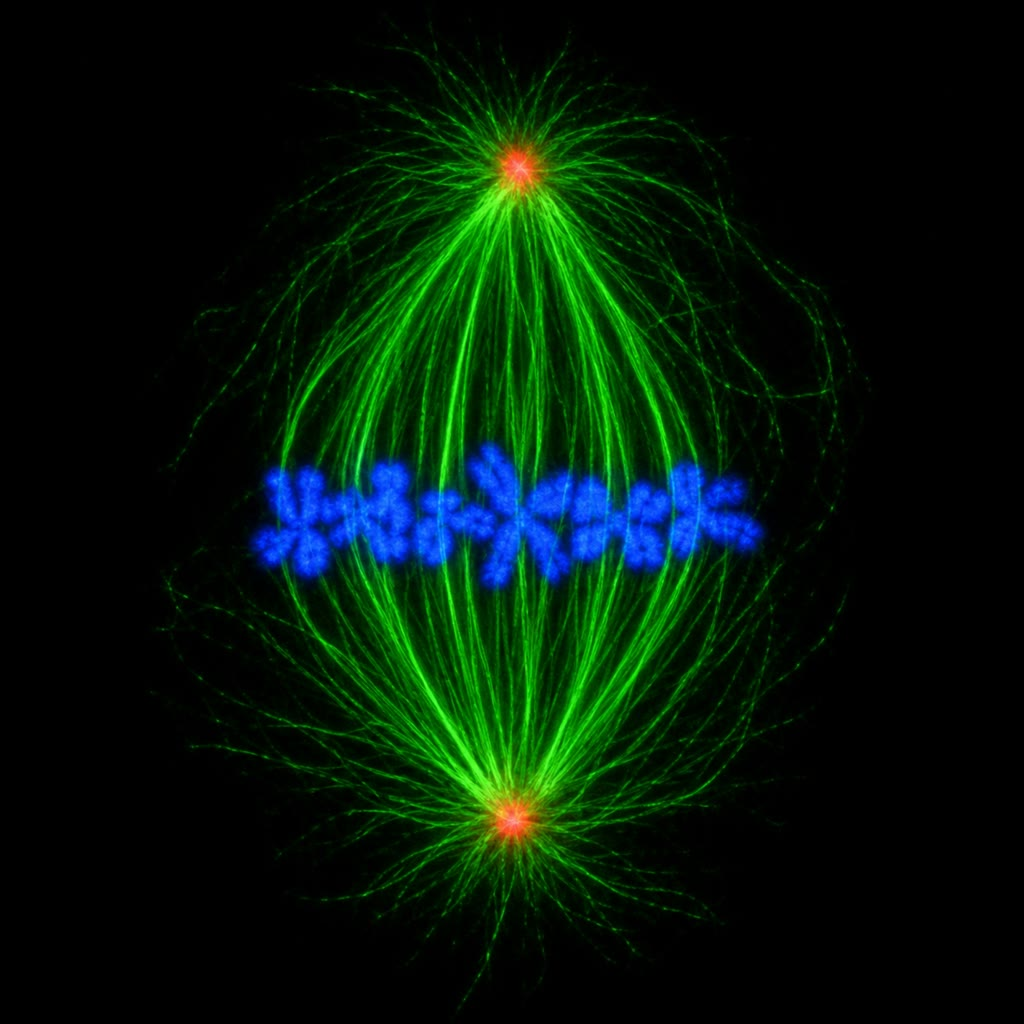
\includegraphics[width=0.36\linewidth]{images/book5/ai/b5-10-mitotic-spindle.jpg}\hspace{0.04\linewidth}
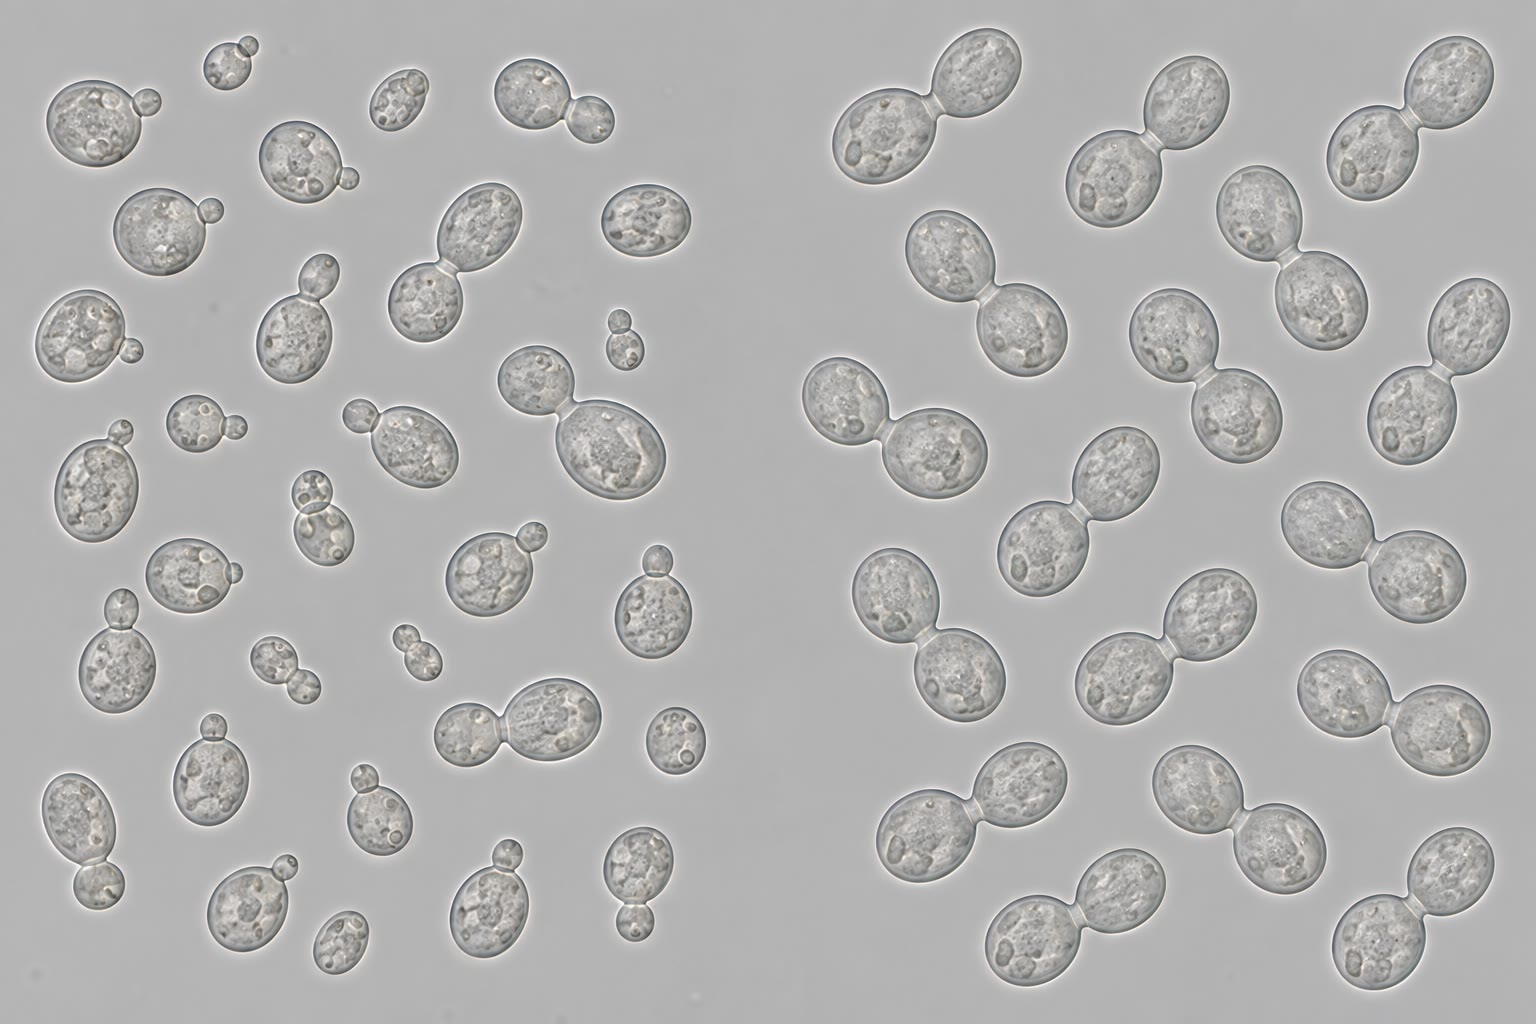
\includegraphics[width=0.54\linewidth]{images/book5/ai/b5-10-yeast-cdc-mutants.jpg}

{\small À esquerda: uma célula em metáfase --- \omterm{def:b3:cytoskeleton-motility:filaments}{microtúbulos} do fuso
(verde) vindos dos dois polos (vermelho), cromossomos (azul) alinhados
na placa, o momento em que o \omterm{def:b3:cell-cycle-apoptosis:checkpoints}{ponto de checagem} do fuso decide. À
direita: levedura de brotamento, do tipo selvagem com brotos de todos
os tamanhos (à esquerda) e um mutante \emph{cdc} em que cada célula
parou na mesma etapa, cada uma com um broto do mesmo tamanho (à
direita).}
\end{omfigure}

\section{Apoptose}

\begin{definition}[Apoptose]\label{def:b3:cell-cycle-apoptosis:apoptosis}
\index{apoptose}\index{necrose}\index{caspase}\index{fosfatidilserina}
A \emph{apoptose} é a morte celular programada por uma sequência
intrínseca: a célula encolhe e se arredonda, sua \omterm{def:b3:chromatin-epigenetics:nucleosome}{cromatina} se condensa
e seu DNA é cortado entre os \omterm{def:b3:chromatin-epigenetics:nucleosome}{nucleossomos} numa escada de fragmentos, o
núcleo se desfaz, a membrana forma bolhas seladas, a fosfatidilserina
aparece na face externa da membrana como um sinal de ``coma-me'', e os
fragmentos são englobados por vizinhos ou por macrófagos em menos de
uma hora --- sem vazamento e, portanto, sem inflamação. Ela é executada
pelas \emph{caspases}, proteases de cisteína que cortam depois de um
aspartato, feitas como zimogênios inativos: as caspases
\emph{iniciadoras} (8 e 9) são ativadas por serem reunidas numa
plataforma, e clivam e ativam as caspases \emph{executoras} (3 e 7),
que cortam várias centenas de substratos --- as lâminas, o
citoesqueleto, o inibidor da nuclease que corta o DNA, a enzima que
mantém a fosfatidilserina do lado de dentro. A \emph{necrose}, em
contraste, é a morte por injúria: a célula incha, rompe-se, derrama seu
conteúdo e provoca inflamação. A apoptose foi nomeada e sua morfologia
descrita por Kerr, Wyllie e Currie (1972); seus genes foram achados num
verme.
\end{definition}

\begin{proof}[Evidência]
Todo hermafrodita de \emph{Caenorhabditis elegans} produz $1090$
células somáticas, das quais as mesmas $131$ morrem, cada uma num
momento e num lugar fixos. Horvitz e colaboradores (anos 1980) isolaram
mutantes em que elas sobreviviam: \emph{ced-3} e \emph{ced-4} eram
necessários a cada morte e, na ausência deles, as $131$ células viviam
e se diferenciavam; \emph{ced-9} protegia --- sua perda matava células
que deveriam ter vivido, e seu excesso de atividade salvava células que
deveriam ter morrido; \emph{egl-1} era necessário a mortes
particulares. A CED-3 era uma \omterm{def:b3:cell-cycle-apoptosis:apoptosis}{caspase}, a CED-4 sua plataforma de
ativação (a Apaf-1 nos humanos), a CED-9 uma proteína Bcl-2, a EGL-1
uma proteína só-BH3: a via humana, gene por gene. O próprio gene humano
\emph{BCL2} havia sido encontrado numa translocação cromossômica no
linfoma folicular, um câncer de células que não morrem.
\end{proof}

\begin{definition}[As duas vias]\label{def:b3:cell-cycle-apoptosis:pathways}
\index{via intrínseca}\index{via extrínseca}\index{família Bcl-2}\index{citocromo c}\index{apoptossomo}\index{receptor de morte}
A via \emph{intrínseca} (mitocondrial) integra o estado interno da
célula. A \emph{família Bcl-2} tem três classes: as guardiãs (Bcl-2,
Bcl-xL, Mcl-1), que se assentam na membrana externa da mitocôndria e a
mantêm selada; as efetoras (Bax, Bak), que, quando ativadas,
oligomerizam em poros nessa membrana; e as sensoras \emph{só-BH3} (Bim,
Bid, Puma, Noxa, Bad), cada uma induzida ou ativada por um insulto
particular --- dano ao DNA pela p53 (Puma, Noxa), retirada de fator de
crescimento (Bim, Bad), desprendimento, proteínas mal enoveladas ---,
que se ligam às guardiãs e liberam ou ativam as efetoras. Quando as
efetoras vencem, a membrana externa é permeabilizada, o
\emph{citocromo~c} vaza para o citosol, liga-se à Apaf-1 e forma o
\emph{apoptossomo}, que ativa a \omterm{def:b3:cell-cycle-apoptosis:apoptosis}{caspase}~9. A via \emph{extrínseca}
começa do lado de fora: os \emph{receptores de morte} (Fas, receptor de
TNF, receptores de TRAIL), ligados por seus ligantes num linfócito
matador ou num vizinho, agrupam-se, recrutam adaptadores e ativam a
\omterm{def:b3:cell-cycle-apoptosis:apoptosis}{caspase}~8, que cliva a \omterm{def:b3:cell-cycle-apoptosis:apoptosis}{caspase}~3 diretamente e, por meio da Bid, também
abre a rota mitocondrial. As duas vias convergem nas \omterm{def:b3:cell-cycle-apoptosis:apoptosis}{caspases}
executoras, e proteínas inibidoras (IAPs, FLIP) fixam o limiar ao longo
do caminho.
\end{definition}

\begin{omfigure}
\begin{tikzpicture}[every node/.style={font=\scriptsize}, >=stealth]
  % extrinsic
  \node[draw, thick, rounded corners, fill=omProp!25, align=center] (lig) at (0,4.2) {ligante de morte numa célula matadora\\(FasL, TNF, TRAIL)};
  \node[draw, thick, rounded corners, fill=omProp!25, align=center] (rec) at (0,2.8) {os receptores de morte se agrupam;\\adaptadores recrutam a caspase-8};
  \node[draw, thick, rounded corners, fill=omThm!20] (c8) at (0,1.5) {caspase-8 ativa};
  % intrinsic
  \node[draw, thick, rounded corners, fill=omDef!20, align=center] (insult) at (7.2,4.2) {dano ao DNA (p53), perda de fator de crescimento,\\desprendimento, proteínas mal enoveladas};
  \node[draw, thick, rounded corners, fill=omDef!20, align=center] (bh3) at (7.2,3.0) {as sensoras só-BH3 (Puma, Bim, Bid)\\neutralizam a Bcl-2 e ativam Bax/Bak};
  \node[draw, thick, rounded corners, fill=omDef!20, align=center] (mito) at (7.2,1.7) {a membrana externa mitocondrial se abre:\\citocromo $c$ para fora, forma-se o apoptossomo};
  \node[draw, thick, rounded corners, fill=omThm!20] (c9) at (7.2,0.5) {caspase-9 ativa};
  % convergence
  \node[draw, thick, rounded corners, fill=omThm!35, align=center] (c3) at (3.6,-0.8) {caspases executoras 3 e 7:\\centenas de substratos cortados};
  \node[draw, thick, rounded corners, fill=gray!15, align=center] (out) at (3.6,-2.3) {cromatina condensada, DNA em escada, bolhas,\\fosfatidilserina exposta, englobada};
  \draw[->, thick] (lig) -- (rec); \draw[->, thick] (rec) -- (c8); \draw[->, thick] (c8) -- (c3);
  \draw[->, thick] (insult) -- (bh3); \draw[->, thick] (bh3) -- (mito); \draw[->, thick] (mito) -- (c9); \draw[->, thick] (c9) -- (c3);
  \draw[->, thick] (c3) -- (out);
  \draw[->, thick, dashed] (c8) -- (bh3) node[pos=0.55, below, sloped] {Bid clivada: as duas rotas se juntam};
  \node[left, omThm, align=right] at (-2.3,1.5) {via\\extrínseca}; \node[right, omDef, align=left] at (10.4,1.7) {via\\intrínseca};
  \node[right, font=\tiny, align=left] at (8.6,0.5) {as IAPs inibem aqui;\\a Bcl-2 guarda acima};
\end{tikzpicture}

{\small As duas rotas até as \omterm{def:b3:cell-cycle-apoptosis:apoptosis}{caspases} executoras. De fora para dentro,
um \omterm{def:b3:cell-cycle-apoptosis:pathways}{receptor de morte} ativa a caspase-8; de dentro para fora, a \omterm{def:b3:cell-cycle-apoptosis:pathways}{família
Bcl-2} pesa o estado da célula e, quando as efetoras vencem, a
mitocôndria libera o citocromo~$c$ e a caspase-9 é ativada. As duas
convergem na caspase-3.}
\end{omfigure}

\begin{proposition}[O ponto sem volta]\label{prop:b3:cell-cycle-apoptosis:mompt}
\index{permeabilização da membrana externa mitocondrial}
A \omterm{prop:b3:cell-cycle-apoptosis:mompt}{permeabilização da membrana externa mitocondrial} é súbita --- todas
as mitocôndrias de uma célula se abrem em cerca de cinco minutos,
depois de horas de deliberação --- e completa: uma vez o citocromo~$c$
no citosol, a ativação das \omterm{def:b3:cell-cycle-apoptosis:apoptosis}{caspases} segue em minutos e não pode ser
desfeita retirando o estímulo. Duas características fazem dela um
interruptor. O poro de Bax/Bak se forma por oligomerização, de modo que
sua taxa sobe abruptamente com a quantidade de efetora ativada; e as
guardiãs e as sensoras se ligam umas às outras com alta afinidade, de
modo que, até um limiar, toda sensora é neutralizada e, além dele, toda
sensora a mais fica livre --- uma titulação, como um tampão que se
esgota. A célula, portanto, não morre aos poucos; ela acumula proteínas
só-BH3 até que um limiar seja cruzado, e então morre de uma vez.
Fármacos que imitam as proteínas BH3 (o venetoclax, que ocupa a Bcl-2)
empurram para além do limiar as células que estão ``preparadas'' ---
já perto dele, como são muitas células leucêmicas ---, poupando as que
não estão.
\end{proposition}

\begin{omfigure}
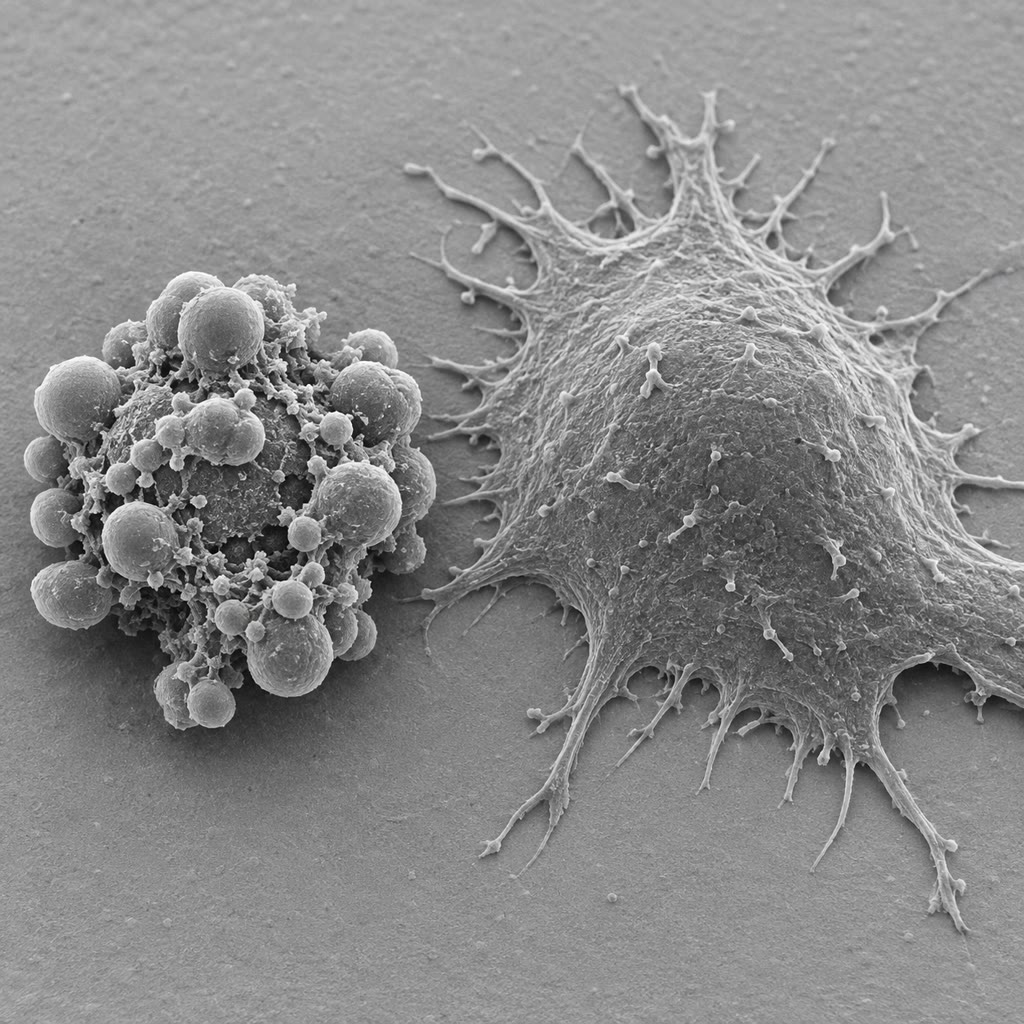
\includegraphics[width=0.40\linewidth]{images/book5/ai/b5-10-apoptotic-cell.jpg}

{\small Uma célula apoptótica ao lado de uma saudável no microscópio
eletrônico de varredura: encolhida, com a superfície quebrada em bolhas
seladas que serão englobadas sem um traço de inflamação.}
\end{omfigure}

\begin{example}[Mortes que constroem um corpo]\label{ex:b3:cell-cycle-apoptosis:development}
Os dedos são esculpidos de uma pá pela \omterm{def:b3:cell-cycle-apoptosis:apoptosis}{apoptose} das células entre eles;
no pato as mesmas células vivem e a membrana permanece. A cauda do
girino é reabsorvida na metamorfose ao sinal do hormônio tireoidiano.
Cerca de metade dos neurônios produzidos no sistema nervoso de um
vertebrado morre antes do nascimento, justamente os que não recebem
fator trófico bastante de seus alvos --- uma competição que ajusta o
número de neurônios ao tamanho do campo que eles servem. Noventa e
cinco por cento dos linfócitos~T feitos no timo morrem ali,
selecionados negativamente por não reconhecerem nada ou por
reconhecerem o próprio corpo (\cref{ch:b3:adaptive-immunity}). E todo
dia o epitélio intestinal descarta suas células mais velhas nas pontas
das vilosidades, a pele seus queratinócitos, o sangue seus neutrófilos
envelhecidos depois de uma vida de um dia: a \omterm{def:b3:cell-cycle-apoptosis:apoptosis}{apoptose} é a rotina, e o
tamanho do tecido é a diferença entre duas taxas grandes.
\end{example}

\section{Outras saídas, e a falha em sair}

\begin{definition}[Necrose regulada e senescência]\label{def:b3:cell-cycle-apoptosis:other}
\index{necroptose}\index{piroptose}\index{senescência}
As células têm outras mortes programadas, todas inflamatórias, ao passo
que a \omterm{def:b3:cell-cycle-apoptosis:apoptosis}{apoptose} é silenciosa. A \emph{necroptose}, disparada por
\omterm{def:b3:cell-cycle-apoptosis:pathways}{receptores de morte} quando a caspase-8 está bloqueada (como alguns
vírus a bloqueiam), monta a cinase RIPK3 com a MLKL, que perfura a
membrana plasmática. A \emph{piroptose}, em macrófagos infectados, é
executada pela caspase-1 do inflamassomo
(\cref{ch:b3:innate-immunity}), que cliva a gasdermina num formador de
poros e libera a interleucina-1. A \emph{ferroptose} é a morte por
peroxidação lipídica dependente de ferro. Uma célula também pode parar
de se dividir sem morrer: a \emph{senescência} é uma parada permanente,
imposta pela p16 e pela p21 depois da erosão dos telômeros
(\cref{ch:b3:stem-cells}), de dano persistente ao DNA ou da ativação de
um oncogene, na qual a célula permanece metabolicamente ativa e secreta
fatores inflamatórios. A senescência remove células danificadas do
conjunto em divisão --- um supressor de tumor --- e se acumula com a
idade, quando suas secreções contribuem para a degeneração dos tecidos;
eliminar células senescentes em camundongos prolonga a vida saudável.
\end{definition}

\begin{remark}[Pouco demais e demais]\label{rem:b3:cell-cycle-apoptosis:disease}
As doenças desses programas são de dose. Morte de menos: o câncer, em
que o limiar apoptótico é elevado pela superexpressão de Bcl-2 ou pela
perda de p53, de modo que células com genomas danificados sobrevivem
para acumular mais dano; a autoimunidade, quando linfócitos que
deveriam ter morrido na seleção persistem. Morte demais: a perda de
linfócitos~T na infecção pelo HIV, os neurônios da penumbra de um
acidente vascular morrendo por \omterm{def:b3:cell-cycle-apoptosis:apoptosis}{apoptose} horas depois da isquemia (uma
janela para tratamento), a \omterm{def:b3:cell-cycle-apoptosis:apoptosis}{apoptose} lenta de neurônios nas doenças
neurodegenerativas, as células cardíacas perdidas depois de um infarto.
O tratamento do câncer é, em grande medida, a indução deliberada de
\omterm{def:b3:cell-cycle-apoptosis:apoptosis}{apoptose} em células cujos limiares são mais baixos que os das vizinhas,
e os fármacos que miram a Bcl-2 e a Cdk4/6 são os primeiros projetados
a partir dos mapas deste capítulo.
\end{remark}

\section{Exercícios}

\begin{exercise}[$\star$]\label{exo:b3:cell-cycle-apoptosis:1}
Liste as quatro fases do ciclo, o par ciclina--CDK que impulsiona cada
transição e a ubiquitina-ligase que encerra a mitose.
\end{exercise}

\begin{exercise}[$\star$]\label{exo:b3:cell-cycle-apoptosis:2}
Com que cada um de Hartwell, Nurse e Hunt contribuiu para a descoberta
do motor, e em que organismo?
\end{exercise}

\begin{exercise}[$\star$]\label{exo:b3:cell-cycle-apoptosis:3}
Nomeie os três \omterm{def:b3:cell-cycle-apoptosis:checkpoints}{pontos de checagem}, a condição que cada um testa e o
alvo molecular sobre o qual cada um age.
\end{exercise}

\begin{exercise}[$\star$]\label{exo:b3:cell-cycle-apoptosis:4}
Distinga a \omterm{def:b3:cell-cycle-apoptosis:apoptosis}{apoptose} da \omterm{def:b3:cell-cycle-apoptosis:apoptosis}{necrose} em cinco características, e nomeie a
classe de enzimas que executa a \omterm{def:b3:cell-cycle-apoptosis:apoptosis}{apoptose}.
\end{exercise}

\begin{exercise}[$\star\star$]\label{exo:b3:cell-cycle-apoptosis:5}
Num extrato de óvulo de rã a \omterm{def:b3:cell-cycle-apoptosis:cdk}{ciclina} B é sintetizada a $k_{s} = 1$
unidade por minuto; o limiar mitótico é $C_{2} = 30$ unidades, o limiar
de saída é $C_{1} = 5$, e na mitose a \omterm{def:b3:cell-cycle-apoptosis:cdk}{ciclina} é degradada com meia-vida
de \qty{2}{min}. Estime o período da oscilação e a fração do ciclo
passada em mitose.
\end{exercise}

\begin{exercise}[$\star\star$]\label{exo:b3:cell-cycle-apoptosis:6}
Preveja o comportamento de uma célula (a) que expressa uma \omterm{def:b3:cell-cycle-apoptosis:cdk}{ciclina} B
não degradável, (b) sem Wee1, (c) sem Cdc25, (d) que expressa uma Cdk1
que não pode ser fosforilada pela Wee1, em termos do oscilador do
\cref{thm:b3:cell-cycle-apoptosis:oscillator}.
\end{exercise}

\begin{exercise}[$\star\star$]\label{exo:b3:cell-cycle-apoptosis:7}
Uma fusão de Rao--Johnson junta uma célula em G1 a uma célula em fase
S; outra junta uma célula em G2 a uma em fase S. Preveja o que cada
núcleo faz e explique com o licenciamento e os níveis de CDK.
\end{exercise}

\begin{exercise}[$\star\star$]\label{exo:b3:cell-cycle-apoptosis:8}
Explique por que um único cinetócoro não ligado consegue segurar a
anáfase da célula inteira, e preveja o destino de uma célula em que a
Mad2 foi deletada.
\end{exercise}

\begin{exercise}[$\star\star$]\label{exo:b3:cell-cycle-apoptosis:9}
Preveja o fenótipo de um verme sem \emph{ced-9}; sem \emph{ced-3}; sem
os dois. Explique a epistasia em termos da via.
\end{exercise}

\begin{exercise}[$\star\star\star$]\label{exo:b3:cell-cycle-apoptosis:10}
Mostre que uma única alça de retroalimentação negativa sem interruptor
biestável --- \omterm{def:b3:cell-cycle-apoptosis:cdk}{ciclina} sintetizada a $k_{s}$, degradada a $k_{d}AC$ com
$A$ simplesmente proporcional a $C$ --- tem um estado estacionário
estável e não oscila. O que a curva em S acrescenta, e o que um atraso
acrescentaria em seu lugar?
\end{exercise}

\begin{exercise}[$\star\star\star$]\label{exo:b3:cell-cycle-apoptosis:11}
Uma célula tem $N$ moléculas da guardiã Bcl-2 e recebe sensoras só-BH3
a uma taxa $r$ por hora depois de um estímulo danoso, cada sensora
ligando uma guardiã. Explique por que a célula morre por volta do
instante $N/r$ seja qual for a intensidade do estímulo além disso, por
que a morte é súbita, e o que o venetoclax faz a esse tempo.
\end{exercise}

\begin{exercise}[$\star\star\star$]\label{exo:b3:cell-cycle-apoptosis:12}
O linfoma folicular carrega uma translocação que superexpressa o
\emph{BCL2}; suas células se dividem devagar. O retinoblastoma carrega
a perda do \emph{RB}; suas células se dividem depressa. Explique como
cada lesão isolada produz um tumor, por que o primeiro é indolente e o
segundo agressivo, e o que cada um diz sobre os dois programas deste
capítulo.
\end{exercise}

\section{Problema: a vida e a morte de um epitélio}

\begin{problem}[{Problema de fim de semana --- o revestimento intestinal
renovado célula a célula, o ciclo cronometrado pelo oscilador de
ciclina, os erros de um ponto de checagem contados por todo o corpo e o
descarte apoptótico de cem bilhões de células por dia pesado,
terminando no período do ciclo, nas células aneuploides produzidas por
dia e na massa que o corpo recicla por apoptose}]
\label{pb:b3:cell-cycle-apoptosis:1}
Dados: o intestino delgado tem $10^{7}$ criptas, cada uma renovando uma
vilosidade de \num{3500} células a cada $5$ dias; cada cripta abriga
cerca de $22$ células-tronco que se dividem uma vez por dia, e cuja
progênie se divide mais $5$ vezes antes de se diferenciar. Oscilador:
$k_{s} = 2$ unidades de \omterm{def:b3:cell-cycle-apoptosis:cdk}{ciclina} por hora, $C_{2} = 40$ unidades,
$C_{1} = 8$, meia-vida da \omterm{def:b3:cell-cycle-apoptosis:cdk}{ciclina} mitótica \qty{10}{min}. \omterm{def:b3:cell-cycle-apoptosis:checkpoints}{Ponto de
checagem}: sem o \omterm{def:b3:cell-cycle-apoptosis:checkpoints}{ponto de checagem} do fuso, uma divisão em $50$ segrega
mal um cromossomo; com ele, uma em \num{50000}. O corpo substitui
$10^{11}$ células por dia, de massa \qty{1}{ng} cada, com proteína
correspondendo a \qty{20}{\%} da massa; um macrófago limpa uma célula
apoptótica em \qty{1}{h}.

\medskip
\noindent\textbf{Parte I --- Renovação.}
\begin{enumerate}
  \item Quantas células o intestino delgado descarta por dia, e por
        segundo?
  \item Quantas células uma cripta produz por dia? Confira: $22$
        divisões de células-tronco por dia, cada filha comprometida se
        dividindo mais $5$ vezes.
  \item Se uma célula-tronco se divide uma vez por dia durante uma vida
        de $80$ anos, quantas divisões? Com uma taxa de mutação de
        $0.6$ por genoma por divisão (\cref{ch:b3:dna-repair}), quantas
        mutações ela acumula?
  \item As células de trânsito se dividem a cada \qty{12}{h}. Por que o
        tecido pode se dar ao luxo de divisões de trânsito rápidas e de
        vida curta, mas mantém a célula-tronco lenta?
  \item Uma dose de radiação mata todas as células de trânsito em
        divisão, mas poupa as células-tronco, que retomam em um dia.
        Quanto tempo até a vilosidade, sem reposição, ficar nua, e
        quanto tempo para reconstruí-la? Por que o intestino é uma das
        primeiras vítimas da radiação?
  \item No cólon o descarte no topo se dá por \omterm{def:b3:cell-cycle-apoptosis:apoptosis}{apoptose} (anoikis, morte
        por desprendimento). Por que esse é o modo de morte certo para
        uma célula em contato com as bactérias do intestino?
\end{enumerate}

\medskip
\noindent\textbf{Parte II --- O relógio.}
\begin{enumerate}[resume]
  \item Com os dados do oscilador, quanto tempo a \omterm{def:b3:cell-cycle-apoptosis:cdk}{ciclina} leva para
        subir de $C_{1}$ a $C_{2}$?
  \item Quanto tempo a degradação mitótica leva para trazê-la de
        $C_{2}$ de volta a $C_{1}$?
  \item Período do oscilador nu, e fração do período passada com a Cdk1
        ativa.
  \item As células de trânsito da cripta ciclam em \qty{12}{h}, as
        células-tronco em \qty{24}{h}, o óvulo de rã em \qty{30}{min}.
        Qual dos parâmetros do modelo difere, e o que fornece a
        diferença numa célula somática?
  \item Uma célula parada no \omterm{def:b3:cell-cycle-apoptosis:checkpoints}{ponto de checagem} G2/M por dano ao DNA
        continua produzindo \omterm{def:b3:cell-cycle-apoptosis:cdk}{ciclina} B. Onde ela está no plano de fase, e
        o que a mantém ali? O que acontece quando o dano é reparado?
  \item Um fármaco inibe o APC/C. Descreva o destino de uma célula que
        entre em mitose na presença dele.
\end{enumerate}

\medskip
\noindent\textbf{Parte III --- Erros.}
\begin{enumerate}[resume]
  \item Quantas divisões por dia o corpo realiza para substituir
        $10^{11}$ células?
  \item Quantas filhas aneuploides por dia com o \omterm{def:b3:cell-cycle-apoptosis:checkpoints}{ponto de checagem}, e
        sem ele?
  \item A maioria das células aneuploides morre ou para (a p53 responde
        à má segregação). Se \qty{1}{\%} sobrevive e se divide, quantas
        células aneuploides em divisão um corpo com \omterm{def:b3:cell-cycle-apoptosis:checkpoints}{ponto de checagem}
        competente produz por dia, e ao longo de uma vida?
  \item Um tumor de $10^{9}$ células perdeu o \omterm{def:b3:cell-cycle-apoptosis:checkpoints}{ponto de checagem} e a
        p53. Quantas más segregações por dia ele realiza, e por que
        isso o faz evoluir depressa?
  \item Explique por que a perda completa do \omterm{def:b3:cell-cycle-apoptosis:checkpoints}{ponto de checagem} do fuso é
        letal para um embrião, embora a perda parcial promova o câncer.
  \item A síndrome de Down surge de uma má segregação na meiose, não na
        mitose. Explique por que um erro numa única célula ali afeta
        cada célula da criança, ao passo que um erro mitótico afeta uma
        linhagem.
\end{enumerate}

\medskip
\noindent\textbf{Parte IV --- Descarte.}
\begin{enumerate}[resume]
  \item Que massa de células o corpo descarta por \omterm{def:b3:cell-cycle-apoptosis:apoptosis}{apoptose} por dia, e
        por ano? Compare com a massa corporal.
  \item Quanta proteína é isso por dia? Compare com uma ingestão
        alimentar de \qty{70}{g}: que fração da renovação proteica do
        corpo é a reciclagem das células mortas?
  \item Quantos macrófagos, trabalhando sem parar, são necessários para
        limpar os mortos do dia? O corpo tem cerca de $10^{11}$
        macrófagos: que fração do tempo deles?
  \item Por que o corpo precisa ser removido antes de se lisar, e o que
        sinaliza ``coma-me''?
  \item A Bcl-2 de um paciente está superexpressa em linfócitos~B. Qual
        via está bloqueada, a \omterm{def:b3:cell-cycle-apoptosis:pathways}{via extrínseca} ainda funciona, e por que o
        resultado é um linfoma de crescimento lento, e não rápido?
  \item Os neurônios da penumbra de um acidente vascular morrem por
        \omterm{def:b3:cell-cycle-apoptosis:apoptosis}{apoptose} de seis a vinte e quatro horas depois do insulto, e os
        do núcleo por \omterm{def:b3:cell-cycle-apoptosis:apoptosis}{necrose} em minutos. Por que o primeiro caso
        oferece uma janela para tratamento e o segundo não?
  \item Resuma: o período do oscilador nu (questão~9), as células
        aneuploides em divisão por dia num corpo normal (questão~15) e a
        massa reciclada por \omterm{def:b3:cell-cycle-apoptosis:apoptosis}{apoptose} por dia (questão~19).
\end{enumerate}
\end{problem}
